\documentclass[a4paper,12pt,oneside]{book}
\linespread{1.5}
\usepackage{geometry}
\geometry{top=2cm,bottom=2.5cm,left=3.5cm,right=3.5cm} % Impostiamo il valore dei margini.
\usepackage[utf8]{inputenc}
\usepackage[T1]{fontenc}
\usepackage{lmodern}
\usepackage{microtype}
\usepackage[italian]{babel} %% Abbiamo istruito LaTeX ad usare la lingua italiana.
\usepackage{subfig}
\setlength{\parindent}{0cm}
\setlength{\emergencystretch}{3em} %% evita righe troppo lunghe con i nomi di file in monospazio

\usepackage{graphicx}
\usepackage{float}
\usepackage{csquotes}
\usepackage{amsmath}
\usepackage{amssymb}
\usepackage{booktabs}
\usepackage{tabularx}
\usepackage{xcolor}
\usepackage{pgfplots}
\usepackage{pgfplotstable}
\usepackage{algorithm}
\usepackage{algpseudocode}
\usepackage{listings}
\usepackage{tocbibind}
\setcounter{tocdepth}{2}
\usepackage[hidelinks]{hyperref}

\usepackage{fancyhdr}
\pagestyle{fancy}
\renewcommand{\headrulewidth}{0pt}
\fancyhf{}
\fancyhead[L]{}
\fancyfoot[C]{\thepage}

\graphicspath{{imgs/}} %% cartella dalla quale ricavare le immagini %%

\pgfplotsset{compat=1.18}
%% Comandi e stili comuni a tutta la relazione %%

%% Colori: serie dei grafici (in ordine fisso) e inchiostri secondari %%
\definecolor{serie1}{HTML}{2A78D6}
\definecolor{serie2}{HTML}{EB6834}
\definecolor{serie3}{HTML}{1BAF7A}
\definecolor{serie4}{HTML}{EDA100}
\definecolor{inchiostro}{HTML}{52514E}
\definecolor{muto}{HTML}{898781}
\definecolor{griglia}{HTML}{E1E0D9}
\definecolor{asse}{HTML}{C3C2B7}
\definecolor{sfondocodice}{HTML}{F5F5F3}

%% Dati dei grafici, ricavati dai risultati dei benchmark da scripts/report_data.py %%
\newcommand{\dati}[1]{dati/#1.csv}

%% Nomi di file, funzioni e opzioni nel testo %%
\newcommand{\codice}[1]{\texttt{#1}}

%% Estratti di codice %%
\lstdefinelanguage{nasm}{
    morekeywords={mov,movsxd,shl,add,sub,neg,jnz,jl,jle,jmp,cmp,test,dec,ret,
        movaps,movss,movd,movdqa,xorps,subps,mulps,addps,haddps,pshufd,fld,
        vmovapd,vsubpd,vmulpd,vaddpd,vxorpd,vhaddpd,vextractf128,vzeroupper,
        vmovd,vpshufd,vinsertf128,vmovdqa},
    morekeywords=[2]{eax,ecx,edx,esp,esi,rdi,rsi,rdx,xmm0,xmm1,ymm0,ymm1,dword},
    morecomment=[l]{;},
    sensitive=false
}
\lstset{
    basicstyle=\ttfamily\footnotesize\linespread{1.0}\selectfont,
    keywordstyle=\color{serie1}\bfseries,
    keywordstyle=[2]\color{serie2},
    commentstyle=\color{muto}\itshape,
    stringstyle=\color{serie3},
    backgroundcolor=\color{sfondocodice},
    frame=single,
    rulecolor=\color{griglia},
    framesep=4pt,
    xleftmargin=4pt,
    xrightmargin=4pt,
    columns=fullflexible,
    keepspaces=true,
    showstringspaces=false,
    breaklines=true,
    tabsize=4,
    captionpos=b,
    literate={è}{{\`e}}1 {à}{{\`a}}1 {ò}{{\`o}}1 {ù}{{\`u}}1 {é}{{\'e}}1 {ì}{{\`i}}1
}
\renewcommand{\lstlistingname}{Listato}
\renewcommand{\lstlistlistingname}{Elenco dei listati}

%% Grafici: griglia e assi recessivi, linee sottili %%
\pgfplotsset{
    relazione/.style={
        width=0.95\textwidth,
        height=0.6\textwidth,
        axis line style={asse},
        tick style={asse},
        grid=major,
        major grid style={griglia, line width=0.4pt},
        tick label style={font=\footnotesize, color=inchiostro},
        label style={font=\small, color=inchiostro},
        legend style={font=\footnotesize, draw=none, fill=none, text=inchiostro},
        legend cell align=left,
        every axis plot/.append style={line width=1.2pt},
        mark size=2.2pt,
    },
}

%% Pseudocodice in italiano %%
\floatname{algorithm}{Algoritmo}
\renewcommand{\listalgorithmname}{Elenco degli algoritmi}
\algrenewcommand\algorithmicrequire{\textbf{Input:}}
\algrenewcommand\algorithmicensure{\textbf{Output:}}
\algrenewcommand\algorithmicif{\textbf{se}}
\algrenewcommand\algorithmicthen{\textbf{allora}}
\algrenewcommand\algorithmicelse{\textbf{altrimenti}}
\algrenewcommand\algorithmicfor{\textbf{per}}
\algrenewcommand\algorithmicforall{\textbf{per ogni}}
\algrenewcommand\algorithmicdo{\textbf{esegui}}
\algrenewcommand\algorithmicwhile{\textbf{finché}}
\algrenewcommand\algorithmicreturn{\textbf{restituisci}}
\algrenewcommand\algorithmicend{\textbf{fine}}
\algrenewcommand\algorithmicfunction{\textbf{funzione}}
\algrenewcommand\algorithmicprocedure{\textbf{procedura}}
\algrenewtext{EndIf}{\algorithmicend\ \algorithmicif}
\algrenewtext{EndFor}{\algorithmicend\ \algorithmicfor}
\algrenewtext{EndWhile}{\algorithmicend\ \algorithmicwhile}
\algrenewtext{EndFunction}{\algorithmicend\ \algorithmicfunction}
\algrenewtext{EndProcedure}{\algorithmicend\ \algorithmicprocedure}

%% Righe di tabella generate da scripts/report_data.py: \input non si può usare dentro tabular %%
\makeatletter
\newcommand{\tabella}[1]{\@@input tabelle/#1.tex }
\makeatother


\begin{document}
%% Frontespizio %%
\begin{titlepage}
    \begin{center}
    \vspace*{0.2cm}
    \begin{figure}[H]
        \centering
        
\includegraphics[width=0.8\textwidth]{imgs/logo.png}
    \end{figure}
        \vspace{5mm}
%% Dipartimento %%
    	\uppercase{\normalsize Dipartimento di Ingegneria Informatica, Modellistica, Elettronica e Sistemistica}\\
    \end{center}
    \begin{center}
%% Corso di Laurea %%
    	\large{Corso di Laurea Magistrale in Ingegneria Informatica}\\
        \vspace{3mm}
        \large{\bf Architetture e Programmazione dei Sistemi di Elaborazione}\\
    	\vspace{10mm}
%% Titolo %%
    {\LARGE{\bf DBSCAN su x86: ottimizzazione con istruzioni SIMD (SSE e AVX) e OpenMP}}\\
     \vspace{7mm}
    \end{center}

    \vspace{25mm}
    \noindent
    \begin{minipage}[t]{0.47\textwidth}
%% Docente %%
    	{\large{\bf Prof. \\Fabrizio Angiulli}}
    	\vspace{12mm}
    \end{minipage}
    \hfill
    \begin{minipage}[t]{0.4\textwidth}\raggedleft
%% Studenti %%
    	{\large{\bf Gabriele Hamil \\ Giovanni Pascuzzi}}
    \end{minipage}

    \vspace{30mm}

%% Anno Accademico %%
    \centering{\large \uppercase{Anno Accademico 23/24}}

\end{titlepage}

%% Corpo della relazione %%
\tableofcontents
\listoffigures
\listoftables
\chapter{Sommario e Introduzione}

\section{Descrizione del Progetto}

Il progetto consiste nell'implementazione dell'algoritmo di clustering \textbf{DBSCAN}~\cite{ester1996} in linguaggio C e assembly x86 e nella sua ottimizzazione su due fronti: il parallelismo a livello di dato, ottenuto con le istruzioni \textbf{SIMD} delle estensioni SSE e AVX, e il parallelismo a livello di thread, ottenuto con \textbf{OpenMP}. Il lavoro è stato svolto per il corso di Architetture e Programmazione dei Sistemi di Elaborazione, a partire dal template fornito dal docente, che stabilisce il formato dei dati di ingresso e i vincoli tecnologici: una versione a 32 bit in singola precisione con istruzioni SSE e una versione a 64 bit in doppia precisione con istruzioni AVX, ciascuna con e senza OpenMP.

\subsection*{Il problema}

DBSCAN raggruppa i punti di un dataset in base alla densità: un punto appartiene a un cluster se nel suo intorno di raggio $\varepsilon$ cadono abbastanza altri punti, e i cluster crescono propagandosi da un punto denso all'altro. A differenza di algoritmi come \emph{k-means}, non richiede di conoscere il numero di cluster, riconosce cluster di forma arbitraria e isola i punti di rumore. Il suo costo è dominato dalle \textbf{interrogazioni di vicinato}: per ogni punto occorre trovare tutti i punti entro distanza $\varepsilon$, e una ricerca esaustiva richiede $n^2$ calcoli di distanza. Sono quindi tre le leve su cui agire:

\begin{enumerate}
    \item \textbf{calcolare meno distanze}, con una struttura dati spaziale che escluda in blocco le regioni lontane dal punto interrogato: in questo progetto un \emph{Ball Tree};
    \item \textbf{calcolare ogni distanza più in fretta}, elaborando più coordinate con una sola istruzione SIMD;
    \item \textbf{calcolare più distanze contemporaneamente}, distribuendo le interrogazioni sui core del processore con OpenMP.
\end{enumerate}

\subsection*{Soluzione adottata}

Il programma legge un dataset in formato binario, esegue DBSCAN e scrive l'etichetta di ogni punto: l'indice del cluster, a partire da 0, oppure $-1$ per il rumore, la stessa convenzione della libreria \emph{scikit-learn}~\cite{sklearn}. Le scelte principali sono le seguenti:

\begin{itemize}
    \item l'algoritmo è riformulato in \textbf{due fasi}: prima si calcolano in parallelo gli intorni di tutti i punti, poi si espandono i cluster in modo sequenziale leggendo gli intorni già calcolati;
    \item le interrogazioni usano un \textbf{Ball Tree}, costruito partizionando sul posto un unico vettore di indici, che esclude le sfere lontane dal punto e accetta in blocco quelle interamente contenute nell'intorno;
    \item le distanze sono calcolate da \textbf{kernel scritti in assembly}, SSE a 32 bit e AVX a 64 bit, su righe del dataset allineate in memoria e completate con zeri fino a un multiplo di quattro valori;
    \item OpenMP distribuisce le interrogazioni della prima fase e la costruzione dell'albero; il tempo è misurato come tempo reale trascorso e non come tempo di CPU.
\end{itemize}

\subsection*{Risultati in sintesi}

Su un dataset di 20.000 punti in 16 dimensioni, con otto cluster e il 5\% di rumore, la versione a 64 bit esegue il clustering in 0,48~s su un singolo thread e in 0,13~s con otto thread, contro 2,03~s della versione consegnata all'esame e 0,36~s di scikit-learn. Le etichette coincidono con quelle di scikit-learn punto per punto su tutti i dataset di prova. Il Capitolo~\ref{cap:sperimentazione} riporta le misure complete.

\subsection*{La versione consegnata e la versione attuale}

La presente relazione descrive la versione del progetto rivista dopo l'esame. La versione consegnata è conservata nel repository con l'etichetta \codice{exam-2024}; la revisione ne ha corretto alcuni errori, tra cui il fatto che OpenMP non venisse mai effettivamente attivato in compilazione, e ne ha ristrutturato il codice. L'Appendice~\ref{app:modifiche} elenca le differenze tra le due versioni.

\section{Organizzazione della Relazione in Capitoli}

Il documento è articolato in otto capitoli, che procedono dall'algoritmo alle scelte implementative e si chiudono con la valutazione sperimentale. Di seguito è fornita una panoramica dei contenuti.

\subsection*{Capitolo 2 --- L'algoritmo DBSCAN}

Il capitolo richiama le definizioni del clustering basato sulla densità e l'algoritmo originale, fissa le convenzioni adottate (etichette, distanza, regola di assegnazione dei punti di confine) e introduce la formulazione in due fasi su cui si basa l'implementazione.

\subsection*{Capitolo 3 --- Architettura del Software e Strutture Dati}

Il capitolo descrive l'organizzazione in moduli, il formato dei file e la disposizione del dataset in memoria, l'array dinamico usato per gli intorni e il Ball Tree, dalla costruzione alle interrogazioni.

\subsection*{Capitolo 4 --- Ottimizzazione mediante Istruzioni SIMD}

Il capitolo presenta i kernel assembly a 32 e a 64 bit, le convenzioni di chiamata che rispettano, i vincoli di allineamento e il confronto con il codice generato dal compilatore.

\subsection*{Capitolo 5 --- Parallelizzazione con OpenMP}

Il capitolo analizza i limiti dell'approccio della versione d'esame e descrive la parallelizzazione adottata: le interrogazioni della prima fase, la costruzione del Ball Tree con i \emph{task} e le ragioni per cui l'espansione resta sequenziale.

\subsection*{Capitolo 6 --- Validazione e Analisi Sperimentale}

Il capitolo verifica la correttezza rispetto a scikit-learn e misura l'effetto di ciascuna ottimizzazione: confronto tra le varianti, scalabilità con i thread e con il numero di punti, dimensione delle foglie del Ball Tree ed effetto della dimensionalità.

\subsection*{Capitolo 7 --- Limiti e Sviluppi Possibili}

Il capitolo discute i limiti della soluzione, a partire dalla memoria occupata dagli intorni, e le ottimizzazioni che non sono state realizzate.

\subsection*{Capitolo 8 --- Conclusioni}

Il capitolo riassume i risultati ottenuti e il contributo di ciascuna tecnica.

\chapter{L'algoritmo DBSCAN}
\label{cap:dbscan}

\section{Clustering Basato sulla Densità}

DBSCAN (\emph{Density-Based Spatial Clustering of Applications with Noise}) è stato proposto da Ester, Kriegel, Sander e Xu nel 1996~\cite{ester1996}. L'idea è che un cluster sia una regione dello spazio in cui i punti sono più densi che nelle regioni circostanti. La densità è misurata con due parametri: il raggio $\varepsilon$ di un intorno e il numero minimo di punti \textit{MinPts} che l'intorno deve contenere. Dato un dataset $D$ e una distanza $\mathrm{dist}$, si definiscono:

\begin{itemize}
    \item l'\textbf{$\varepsilon$-intorno} di un punto $p$: $N_\varepsilon(p) = \{\, q \in D \mid \mathrm{dist}(p, q) \le \varepsilon \,\}$, che comprende $p$ stesso;
    \item \textbf{punto core}: un punto $p$ con $|N_\varepsilon(p)| \ge \mathit{MinPts}$;
    \item \textbf{direttamente raggiungibile}: $q$ è direttamente raggiungibile per densità da $p$ se $p$ è un punto core e $q \in N_\varepsilon(p)$;
    \item \textbf{raggiungibile per densità}: $q$ è raggiungibile da $p$ se esiste una catena $p = p_1, \dots, p_k = q$ in cui ogni punto è direttamente raggiungibile dal precedente;
    \item \textbf{connessi per densità}: $p$ e $q$ sono connessi se esiste un punto $o$ da cui entrambi sono raggiungibili.
\end{itemize}

Un \textbf{cluster} è un insieme non vuoto di punti, massimale rispetto alla raggiungibilità e i cui punti sono a due a due connessi per densità. I punti di un cluster che non sono core si dicono \textbf{punti di confine} (\emph{border}); i punti che non appartengono ad alcun cluster sono \textbf{rumore} (\emph{noise}). Un punto di confine può essere raggiungibile da due cluster diversi: in quel caso l'appartenenza dipende dall'ordine in cui i punti vengono visitati, come osservano gli stessi autori.

\section{L'Algoritmo Originale}

L'Algoritmo~\ref{alg:originale} riporta lo schema del lavoro originale. Si scorrono i punti e, da ogni punto core non ancora classificato, si fa crescere un nuovo cluster con la procedura \textsc{ExpandCluster}, che usa un insieme di \emph{seed} come frontiera di visita: a ogni passo si estrae un seed, si calcola il suo intorno e, se è un punto core, si aggiungono i vicini non ancora visitati.

\begin{algorithm}[H]
\caption{DBSCAN nella formulazione di Ester et al.~\cite{ester1996}}
\label{alg:originale}
\begin{algorithmic}[1]
\Require dataset $D$, raggio $\varepsilon$, soglia \textit{MinPts}
\State $c \gets 0$; tutti i punti sono \textsc{Unclassified}
\ForAll{$p \in D$}
    \If{$p$ è \textsc{Unclassified}}
        \State $S \gets \textsc{RegionQuery}(p, \varepsilon)$
        \If{$|S| < \mathit{MinPts}$}
            \State $p \gets \textsc{Noise}$ \Comment{potrà diventare un punto di confine}
        \Else
            \State assegna $c$ a tutti i punti di $S$; togli $p$ da $S$
            \While{$S \neq \emptyset$}
                \State estrai $q$ da $S$; $R \gets \textsc{RegionQuery}(q, \varepsilon)$
                \If{$|R| \ge \mathit{MinPts}$}
                    \ForAll{$r \in R$ \textsc{Unclassified} o \textsc{Noise}}
                        \State se $r$ è \textsc{Unclassified}, aggiungilo a $S$; assegna $c$ a $r$
                    \EndFor
                \EndIf
            \EndWhile
            \State $c \gets c + 1$
        \EndIf
    \EndIf
\EndFor
\end{algorithmic}
\end{algorithm}

Ogni punto viene interrogato una sola volta, a parte i punti di rumore che rientrano tra i seed di un cluster, quindi il costo complessivo è $O(n \cdot Q)$, dove $Q$ è il costo di una \textsc{RegionQuery}. Con una ricerca esaustiva $Q = O(n\,d)$ e l'algoritmo diventa quadratico nel numero di punti. Con un indice spaziale $Q$ scende, nei casi favorevoli, a un costo logaritmico più la dimensione dell'intorno; Schubert et al.~\cite{schubert2017} mostrano però che questo vale solo se $\varepsilon$ è piccolo rispetto alla scala dei dati, perché con intorni grandi la dimensione stessa dei risultati rende il costo quadratico.

\section{Convenzioni Adottate}

\subsection*{Etichette}

Il risultato è un vettore di interi con un'etichetta per punto: l'indice del cluster, numerato da 0 nell'ordine in cui i cluster vengono scoperti, oppure $-1$ (\codice{NOISE}) per il rumore. Durante l'elaborazione il valore $-2$ (\codice{UNCLASSIFIED}) indica un punto non ancora raggiunto. È la stessa convenzione di scikit-learn~\cite{sklearn}, il che permette di confrontare i risultati direttamente.

\subsection*{Il parametro MinPts}

\textit{MinPts} conta anche il punto stesso, come nella definizione di $\varepsilon$-intorno e come il parametro \codice{min\_samples} di scikit-learn. Internamente le interrogazioni restituiscono l'intorno \emph{senza} il punto interrogato, che non servirebbe in alcun passo successivo, e la condizione di punto core diventa quindi $|N_\varepsilon(p) \setminus \{p\}| + 1 \ge \mathit{MinPts}$.

\subsection*{Distanza euclidea e confronti al quadrato}

La distanza è quella euclidea, indotta dalla norma~2, in accordo con scikit-learn. Poiché la radice quadrata è monotona crescente, $\mathrm{dist}(p,q) \le \varepsilon$ equivale a $\mathrm{dist}(p,q)^2 \le \varepsilon^2$: i kernel calcolano quindi la \textbf{distanza al quadrato} e la radice viene estratta solo dove serve una distanza vera, cioè nel Ball Tree per i raggi delle sfere e per i test di esclusione. Una norma diversa, per esempio la norma~1 (distanza di Manhattan), individuerebbe intorni diversi e quindi cluster diversi: i risultati non sarebbero più confrontabili con quelli di riferimento.

\subsection*{Assegnazione dei punti di confine}

Quando un punto di confine è raggiungibile da più cluster, l'implementazione lo assegna al \textbf{primo} cluster che lo raggiunge, come scikit-learn. L'Algoritmo~\ref{alg:originale}, invece, assegna al nuovo cluster tutti i punti dell'intorno iniziale, anche quelli già attribuiti a un cluster precedente. Entrambe le scelte sono legittime, ma la prima rende il risultato identico a quello di scikit-learn e quindi verificabile in modo esatto.

\section{Formulazione in Due Fasi}
\label{sec:due-fasi}

Nell'Algoritmo~\ref{alg:originale} le interrogazioni sono intrecciate con l'espansione: quale punto interrogare dopo dipende dal risultato delle interrogazioni precedenti. Questo lascia poco spazio al parallelismo, che nella versione d'esame era stato cercato all'interno delle singole interrogazioni (Capitolo~\ref{cap:openmp}). L'implementazione separa invece il lavoro in due fasi (Algoritmo~\ref{alg:due-fasi}):

\begin{enumerate}
    \item \textbf{Fase 1, intorni}: si calcola l'intorno di ogni punto e si stabilisce se è un punto core. Le interrogazioni sono indipendenti tra loro e possono essere eseguite in parallelo. Si conservano solo gli intorni dei punti core, gli unici che l'espansione leggerà.
    \item \textbf{Fase 2, espansione}: i cluster crescono con una visita in profondità del grafo che ha per nodi i punti e per archi le relazioni di raggiungibilità diretta, usando una pila. Nessuna distanza viene più calcolata.
\end{enumerate}

\begin{algorithm}[H]
\caption{DBSCAN in due fasi, come implementato in \codice{src/dbscan.c}}
\label{alg:due-fasi}
\begin{algorithmic}[1]
\Require dataset $D$ di $n$ punti, raggio $\varepsilon$, soglia \textit{MinPts}
\Ensure etichette $L[0..n)$
\ForAll{$p \in D$} \Comment{Fase 1, in parallelo}
    \State $N[p] \gets \textsc{RegionQuery}(p, \varepsilon) \setminus \{p\}$
    \State $\mathit{core}[p] \gets |N[p]| + 1 \ge \mathit{MinPts}$
    \If{\textbf{non} $\mathit{core}[p]$} \State scarta $N[p]$ \EndIf
\EndFor
\State $L \gets$ \textsc{Unclassified}; $c \gets 0$ \Comment{Fase 2, sequenziale}
\For{$p \gets 0$ \textbf{to} $n-1$}
    \If{$L[p] =$ \textsc{Unclassified} \textbf{e} $\mathit{core}[p]$}
        \State $L[p] \gets c$; inserisci $p$ nella pila
        \While{la pila non è vuota}
            \State $q \gets$ estrai dalla pila \Comment{sempre un punto core}
            \ForAll{$r \in N[q]$ con $L[r] =$ \textsc{Unclassified}}
                \State $L[r] \gets c$
                \If{$\mathit{core}[r]$} \State inserisci $r$ nella pila \EndIf
            \EndFor
        \EndWhile
        \State $c \gets c + 1$
    \EndIf
\EndFor
\State i punti rimasti \textsc{Unclassified} diventano \textsc{Noise}
\end{algorithmic}
\end{algorithm}

La seconda fase produce gli stessi cluster dell'algoritmo originale: un cluster nasce dal primo punto core non ancora etichettato, nello stesso ordine di scansione, e contiene tutti i punti raggiungibili da esso, perché la visita prosegue solo attraverso i punti core ed etichetta ogni loro vicino. Anche il numero di interrogazioni resta lo stesso, una per punto. Il prezzo è la memoria: gli intorni dei punti core restano in memoria fino alla fine, per un totale proporzionale alla somma delle loro dimensioni. È la stessa scelta di scikit-learn, che calcola tutti gli intorni prima dell'espansione, e se ne discutono i limiti nel Capitolo~\ref{cap:limiti}.

\chapter{Architettura del Software e Strutture Dati}
\label{cap:architettura}

\section{Organizzazione dei Moduli}

Il codice è un unico insieme di sorgenti C11 e assembly NASM, organizzato in moduli con responsabilità distinte (Figura~\ref{fig:architettura}). Le quattro varianti richieste dal corso non sono più quattro copie del programma, come nella versione d'esame, ma quattro compilazioni degli stessi sorgenti, prodotte dal \codice{Makefile} (Tabella~\ref{tab:varianti}): la precisione dipende dall'architettura di destinazione, attraverso il tipo \codice{real\_t} definito in \codice{common.h}, e OpenMP si attiva con l'opzione \codice{-fopenmp} del compilatore. Senza di essa le direttive \codice{\#pragma omp} vengono ignorate e il programma resta sequenziale.

\begin{figure}[H]
    \centering
    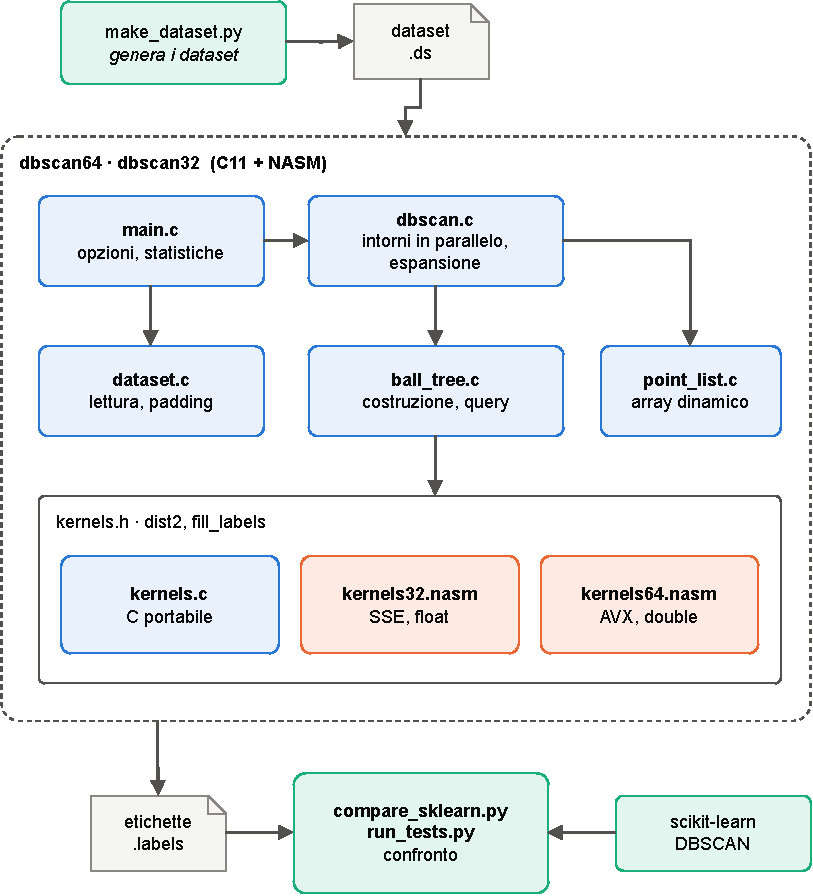
\includegraphics[width=0.85\textwidth]{diagrammi/architettura.pdf}
    \caption{Moduli del programma e strumenti di supporto. In blu i moduli C, in arancione i kernel assembly, in verde gli script Python.}
    \label{fig:architettura}
\end{figure}

\begin{table}[H]
    \centering
    \small
    \begin{tabular}{llll}
        \toprule
        \textbf{Eseguibile} & \textbf{Architettura} & \textbf{Precisione e kernel} & \textbf{OpenMP} \\
        \midrule
        \codice{dbscan32}     & x86-32 & \codice{float}, SSE  & no \\
        \codice{dbscan32-omp} & x86-32 & \codice{float}, SSE  & sì \\
        \codice{dbscan64}     & x86-64 & \codice{double}, AVX & no \\
        \codice{dbscan64-omp} & x86-64 & \codice{double}, AVX & sì \\
        \bottomrule
    \end{tabular}
    \caption{Le quattro varianti prodotte da \codice{make}.}
    \label{tab:varianti}
\end{table}

I moduli sono i seguenti:

\begin{itemize}
    \item \codice{main.c}: interpreta la riga di comando, carica il dataset, invoca l'algoritmo e stampa le statistiche, anche in formato JSON per gli script di misura;
    \item \codice{dataset.c}: legge i file, converte i valori in \codice{real\_t}, completa le righe con zeri e le allinea in memoria; scrive le etichette;
    \item \codice{dbscan.c}: l'algoritmo in due fasi della Sezione~\ref{sec:due-fasi} e la ricerca esaustiva;
    \item \codice{ball\_tree.c}: costruzione e interrogazione del Ball Tree;
    \item \codice{point\_list.c}: l'array dinamico di indici usato per gli intorni e come pila;
    \item \codice{kernels.h}: l'interfaccia dei due kernel, la distanza al quadrato \codice{dist2} e il riempimento delle etichette \codice{fill\_labels}, con una versione in C (\codice{kernels.c}) e una in assembly per ciascuna architettura (\codice{asm/kernels32.nasm} e \codice{asm/kernels64.nasm}). La versione da usare è scelta all'avvio tramite un puntatore a funzione, così che le due si possano confrontare con lo stesso eseguibile.
\end{itemize}

Accanto al programma, alcuni script Python completano il progetto:
\begin{itemize}
    \item \codice{make\_dataset.py} genera i dataset;
    \item \codice{compare\_sklearn.py} e \codice{tests/run\_tests.py} confrontano le etichette con quelle di scikit-learn;
    \item \codice{benchmark.py} esegue le misure del Capitolo~\ref{cap:sperimentazione}, e \codice{report\_data.py} ne ricava tabelle e grafici.
\end{itemize}

\section{Formato dei File e Disposizione in Memoria}

\subsection*{Formato dei file}

Il formato è quello del template del corso: due interi a 32 bit, il numero di colonne e il numero di righe, seguiti dai valori della matrice riga per riga (\emph{row-major order}). I valori sono numeri in virgola mobile a 32 o a 64 bit; il programma deduce la precisione dalla dimensione del file e converte i valori nel tipo della propria variante, così lo stesso dataset si può usare con entrambe le architetture. Le etichette sono scritte nello stesso formato, come matrice di una colonna di interi a 32 bit.

\subsection*{Padding e allineamento}
\label{sec:padding}

Le istruzioni SIMD lavorano su blocchi di quattro valori: quattro \codice{float} in un registro XMM a 128 bit o quattro \codice{double} in un registro YMM a 256 bit. Le istruzioni di caricamento allineato (\codice{movaps}, \codice{vmovapd}) richiedono inoltre che l'indirizzo sia multiplo della dimensione del registro, 16 o 32 byte, e generano un'eccezione in caso contrario. Il dataset viene quindi memorizzato come un unico blocco allineato, in cui ogni riga ha un numero di valori, detto \emph{stride}, pari alla dimensione $d$ arrotondata al multiplo di quattro successivo; le colonne aggiunte valgono zero e non alterano le distanze. Poiché la lunghezza di una riga in byte è un multiplo della dimensione di un registro, tutte le righe risultano allineate (Figura~\ref{fig:memoria}), e i kernel possono elaborare ogni riga a blocchi interi senza gestire un residuo.

\begin{figure}[H]
    \centering
    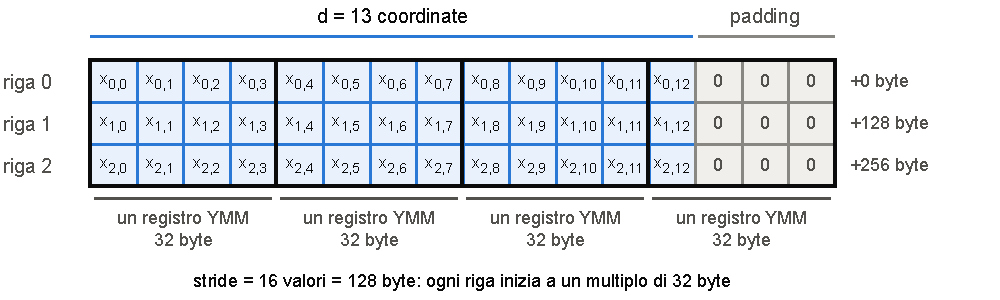
\includegraphics[width=\textwidth]{diagrammi/memoria.pdf}
    \caption{Disposizione in memoria di un dataset con $d = 13$ nella variante a 64 bit: ogni riga è completata con tre zeri fino a 16 valori, cioè 128 byte, e il blocco inizia a un indirizzo multiplo di 32.}
    \label{fig:memoria}
\end{figure}

La versione d'esame otteneva lo stesso risultato con la funzione \codice{adjust\_matrix}, che però allocava una seconda matrice senza liberare la prima; ora il completamento avviene durante la lettura, in un'unica allocazione.

\section{L'Array Dinamico PointList}

Gli intorni hanno dimensioni imprevedibili, da zero a $n-1$ punti. \codice{PointList} è un array di indici che raddoppia la propria capacità quando si riempie: il costo di un inserimento è costante in media, e la memoria sprecata è al più pari a quella usata. La stessa struttura serve da pila nella seconda fase.

Nella versione d'esame questo meccanismo, insieme alla deallocazione esplicita delle liste non più necessarie, era presentato come un sistema di \emph{garbage collection}; si tratta in realtà di gestione manuale della memoria con un array a crescita geometrica. Nella versione attuale ogni thread riusa la stessa \codice{PointList} per tutte le proprie interrogazioni, svuotandola di volta in volta, e copia il risultato in un vettore della dimensione esatta solo se il punto è core: le allocazioni si riducono a una per punto core.

\section{Il Ball Tree}

Un Ball Tree~\cite{omohundro1989} è un albero binario in cui ogni nodo rappresenta una ipersfera, detta \emph{ball}, che contiene un sottoinsieme dei punti: il centro è il centroide dei punti e il raggio è la distanza dal centro al punto più lontano. I due figli di un nodo si spartiscono i suoi punti; le foglie contengono al più \textit{leaf\_size} punti. Rispetto a un \emph{k-d tree}, che divide lo spazio con iperpiani paralleli agli assi, le sfere si adattano meglio alla distribuzione dei dati quando la dimensione cresce.

\begin{figure}[H]
    \centering
    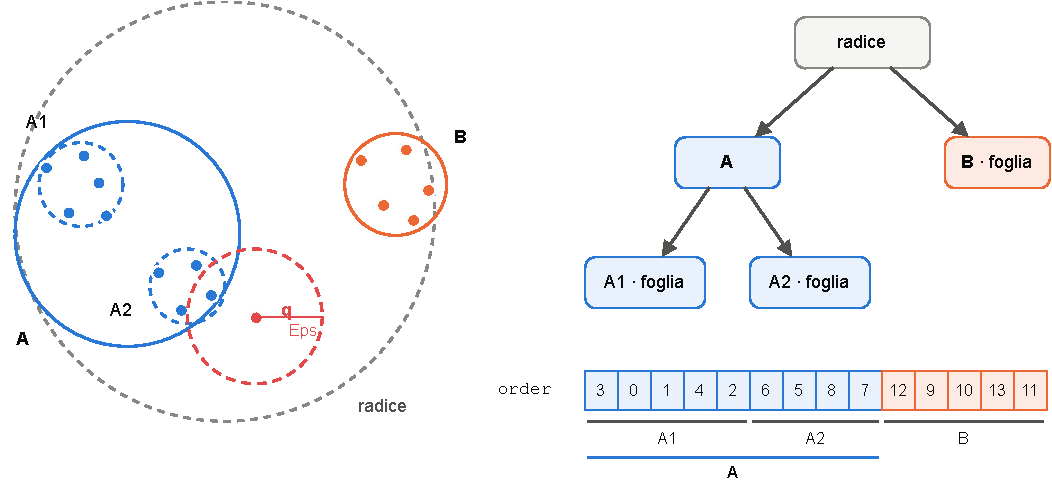
\includegraphics[width=\textwidth]{diagrammi/ball_tree.pdf}
    \caption{A sinistra, un Ball Tree su punti del piano: la radice contiene tutti i punti, i figli \textsf{A} e \textsf{B} ne contengono una parte ciascuno, \textsf{A} è divisa a sua volta in due foglie. L'intorno del punto $q$ interseca \textsf{A} e \textsf{A2}, mentre \textsf{B} viene esclusa senza calcolare alcuna distanza dai suoi punti. A destra, l'albero e il vettore \codice{order}, in cui ogni nodo occupa un intervallo contiguo.}
    \label{fig:balltree}
\end{figure}

\subsection*{Costruzione}

La costruzione parte da un nodo che contiene tutti i punti e lo divide ricorsivamente. Per dividere un nodo si scelgono due punti lontani tra loro: $p_1$, il più lontano dal centroide, e $p_2$, il più lontano da $p_1$. Ogni punto va poi con il più vicino dei due. Il criterio costa due scansioni lineari del nodo e tende a separare i gruppi di punti densi, perché $p_1$ e $p_2$ cadono agli estremi opposti della distribuzione.

L'albero non memorizza liste di punti per nodo. Tutti i nodi condividono un unico vettore di indici, \codice{order}, e la suddivisione ne riordina sul posto l'intervallo con uno schema a due indici simile a quello del \emph{quicksort}: ogni nodo occupa un intervallo contiguo \codice{[start, end)} di \codice{order}, i figli ne occupano le due metà (Figura~\ref{fig:balltree}). Nella versione d'esame ogni nodo allocava invece due nuove liste di punti e liberava quella del padre, con un gran numero di allocazioni. Al termine della costruzione le righe del dataset vengono copiate nell'ordine di \codice{order}: così la scansione di una foglia legge memoria contigua invece di saltare tra righe sparse. La copia raddoppia la memoria occupata dal dataset ma riduce il tempo di esecuzione del 20--40\%, come emerso durante lo sviluppo.

Un nodo diventa foglia quando ha al più \textit{leaf\_size} punti oppure quando tutti i suoi punti coincidono, perché in quel caso il raggio è nullo e nessuna divisione è possibile. La versione d'esame non gestiva questo caso: con più di \textit{leaf\_size} punti identici, tutti finivano nello stesso figlio e la ricorsione non terminava. È presente anche una salvaguardia per il caso, dovuto soltanto agli arrotondamenti, in cui uno dei due figli risulti vuoto.

\subsection*{Interrogazione}

Per trovare l'intorno di un punto $x$ si visita l'albero dalla radice. Per ogni nodo di centro $c$ e raggio $r$ si calcola $\delta = \mathrm{dist}(x, c)$ e, per la disuguaglianza triangolare, si distinguono tre casi:

\begin{enumerate}
    \item se $\delta > r + \varepsilon$, la sfera del nodo e l'intorno di $x$ sono disgiunti: il nodo e tutto il suo sottoalbero vengono esclusi;
    \item se $\delta + r \le \varepsilon$, la sfera è interamente contenuta nell'intorno: tutti i punti del nodo vengono accettati senza calcolarne le distanze;
    \item altrimenti si prosegue sui figli, oppure, in una foglia, si calcola la distanza di ogni punto.
\end{enumerate}

Il secondo caso non era presente nella versione d'esame ed è decisivo quando $\varepsilon$ è grande rispetto alla scala dei dati, come nel dataset usato per l'esame: la Sezione~\ref{sec:caso-esame} mostra che riduce le distanze calcolate da 25 milioni a circa cinquemila. Le distanze dai centri sono le uniche per cui si estrae la radice quadrata, perché i test confrontano somme di distanze; i centroidi sono allocati allineati e completati come le righe del dataset, quindi anche queste distanze usano i kernel SIMD.

\section{Interfaccia a Riga di Comando}

La Tabella~\ref{tab:opzioni} riassume le opzioni del programma. Rispetto al template sono state eliminate le opzioni \codice{-k} e \codice{-labels}, ereditate da un altro progetto del corso e ignorate dall'algoritmo, e sono state aggiunte quelle che selezionano l'indice, i kernel e il numero di thread: le varianti confrontate nel Capitolo~\ref{cap:sperimentazione} si ottengono tutte dallo stesso eseguibile, senza modificare il codice.

\begin{table}[H]
    \centering
    \small
    \begin{tabularx}{\textwidth}{lX}
        \toprule
        \textbf{Opzione} & \textbf{Significato} \\
        \midrule
        \codice{-i}, \codice{--input FILE} & dataset da elaborare \\
        \codice{-e}, \codice{--eps EPS} & raggio $\varepsilon$ dell'intorno \\
        \codice{-m}, \codice{--min-pts N} & soglia \textit{MinPts}, punto stesso incluso \\
        \codice{-o}, \codice{--output FILE} & file in cui scrivere le etichette \\
        \codice{--index KIND} & \codice{balltree} (predefinito) oppure \codice{linear}, la ricerca esaustiva \\
        \codice{--leaf-size N} & punti massimi in una foglia del Ball Tree (predefinito 32) \\
        \codice{--no-simd} & usa i kernel in C invece di quelli SSE/AVX \\
        \codice{-t}, \codice{--threads N} & numero di thread OpenMP (predefinito: tutti i core logici) \\
        \codice{--json} & stampa risultati e tempi come una riga JSON \\
        \codice{-q}, \codice{--quiet} & non stampa nulla oltre agli errori e alla riga JSON \\
        \bottomrule
    \end{tabularx}
    \caption{Opzioni della riga di comando.}
    \label{tab:opzioni}
\end{table}

\chapter{Ottimizzazione mediante Istruzioni SIMD}
\label{cap:simd}

\section{Dove Intervenire}

Quasi tutto il tempo di esecuzione è speso nella prima fase, e al suo interno nel calcolo delle distanze: nelle misure del Capitolo~\ref{cap:sperimentazione} la costruzione del Ball Tree e l'espansione dei cluster pesano insieme meno del 2\% del totale. Il candidato naturale per le istruzioni SIMD (\emph{Single Instruction, Multiple Data}) è quindi il calcolo della distanza al quadrato tra due punti, che applica la stessa sequenza di operazioni --- sottrazione, quadrato, somma --- a tutte le coordinate. Il secondo kernel, il riempimento del vettore delle etichette con un valore costante, è eseguito una sola volta per esecuzione e ha un peso trascurabile; è mantenuto perché era parte dell'esercizio del corso e mostra le istruzioni su dati interi.

Entrambi i kernel sono scritti in assembly NASM, uno per architettura, e dichiarati in \codice{kernels.h} con puntatori e dimensioni come parametri:

\begin{lstlisting}[language=C]
real_t dist2_simd(const real_t *a, const real_t *b, int d);
void fill_labels_simd(int *labels, int n, int value);
\end{lstlisting}

Nella versione d'esame le funzioni assembly ricevevano invece il puntatore alla struttura dei parametri e ne leggevano i campi a spiazzamenti fissi, per esempio \codice{[rdi+40]} per la dimensione: una modifica alla struttura bastava a rompere il codice assembly senza alcun errore di compilazione. Con i puntatori, inoltre, lo stesso kernel serve sia per la distanza tra due righe del dataset sia per quella tra un punto e il centro di una sfera del Ball Tree.

\section{Il Kernel a 32 Bit con SSE}

Nella variante a 32 bit i valori sono \codice{float} e un registro XMM ne contiene quattro. Il Listato~\ref{lst:kernel32} riporta il kernel della distanza.

\begin{lstlisting}[language=nasm, caption={Distanza al quadrato con SSE (\codice{src/asm/kernels32.nasm}).}, label={lst:kernel32}]
dist2_simd:
        mov     eax, [esp+4]            ; a
        mov     ecx, [esp+8]            ; b
        mov     edx, [esp+12]           ; d
        shl     edx, 2                  ; lunghezza della riga in byte
        add     eax, edx                ; puntatori alla fine delle righe,
        add     ecx, edx                ; percorse con uno spiazzamento negativo
        neg     edx
        xorps   xmm0, xmm0              ; 4 somme parziali
.loop:
        movaps  xmm1, [eax+edx]         ; 4 coordinate di a
        subps   xmm1, [ecx+edx]         ; meno 4 coordinate di b
        mulps   xmm1, xmm1
        addps   xmm0, xmm1
        add     edx, 16
        jnz     .loop
        haddps  xmm0, xmm0              ; somma orizzontale (SSE3)
        haddps  xmm0, xmm0
        sub     esp, 4                  ; st(0) si carica solo dalla memoria
        movss   [esp], xmm0
        fld     dword [esp]
        add     esp, 4
        ret
\end{lstlisting}

Alcune scelte meritano un commento:

\begin{itemize}
    \item \textbf{Ciclo a spiazzamento negativo.} I puntatori sono spostati alla fine delle righe e il ciclo le percorre con un indice negativo che cresce fino a zero: l'istruzione \codice{add} che aggiorna l'indice imposta anche il flag di zero, e il ciclo non ha bisogno di un confronto separato.
    \item \textbf{Nessun residuo.} Grazie al padding (Sezione~\ref{sec:padding}) la dimensione è sempre un multiplo di quattro e le righe sono allineate, quindi il ciclo lavora solo su blocchi interi con caricamenti allineati.
    \item \textbf{Somme parziali.} L'accumulatore contiene quattro somme parziali indipendenti, ridotte a una sola alla fine con due \codice{haddps}.
    \item \textbf{Valore di ritorno.} La convenzione di chiamata \emph{cdecl} a 32 bit~\cite{sysv} prevede che una funzione restituisca i valori in virgola mobile in cima allo stack del coprocessore x87, \codice{st(0)}. Non è quindi una scelta, come riportava la relazione d'esame, ma un obbligo. Poiché \codice{st(0)} si può caricare solo dalla memoria, il valore passa per una cella sullo stack del thread. La versione d'esame usava invece una variabile globale: due thread che eseguono il kernel contemporaneamente scrivono nella stessa cella, e uno dei due può restituire la distanza calcolata dall'altro.
    \item \textbf{Registri.} La convenzione impone di preservare \codice{EBX}, \codice{ESI}, \codice{EDI} e \codice{EBP}; il kernel usa solo \codice{EAX}, \codice{ECX}, \codice{EDX} e registri XMM, che il chiamante non si aspetta di ritrovare intatti, e quindi non deve salvare nulla.
\end{itemize}

\section{Il Kernel a 64 Bit con AVX}

Nella variante a 64 bit i valori sono \codice{double} e i registri YMM a 256 bit dell'estensione AVX ne contengono quattro, così che la struttura del ciclo resta la stessa (Listato~\ref{lst:kernel64}). La convenzione di chiamata è quella System V AMD64~\cite{sysv}: i primi argomenti interi arrivano in \codice{RDI}, \codice{RSI} e \codice{RDX}, il risultato in virgola mobile si restituisce in \codice{XMM0}.

\begin{lstlisting}[language=nasm, caption={Distanza al quadrato con AVX (\codice{src/asm/kernels64.nasm}).}, label={lst:kernel64}]
dist2_simd:
        movsxd  rdx, edx
        shl     rdx, 3                  ; lunghezza della riga in byte
        add     rdi, rdx
        add     rsi, rdx
        neg     rdx
        vxorpd  ymm0, ymm0, ymm0        ; 4 somme parziali
.loop:
        vmovapd ymm1, [rdi+rdx]
        vsubpd  ymm1, ymm1, [rsi+rdx]
        vmulpd  ymm1, ymm1, ymm1
        vaddpd  ymm0, ymm0, ymm1
        add     rdx, 32
        jnz     .loop
        vextractf128 xmm1, ymm0, 1      ; somma la meta' alta alla bassa
        vaddpd  xmm0, xmm0, xmm1
        vhaddpd xmm0, xmm0, xmm0        ; e le due corsie rimaste
        vzeroupper
        ret
\end{lstlisting}

\begin{figure}[H]
    \centering
    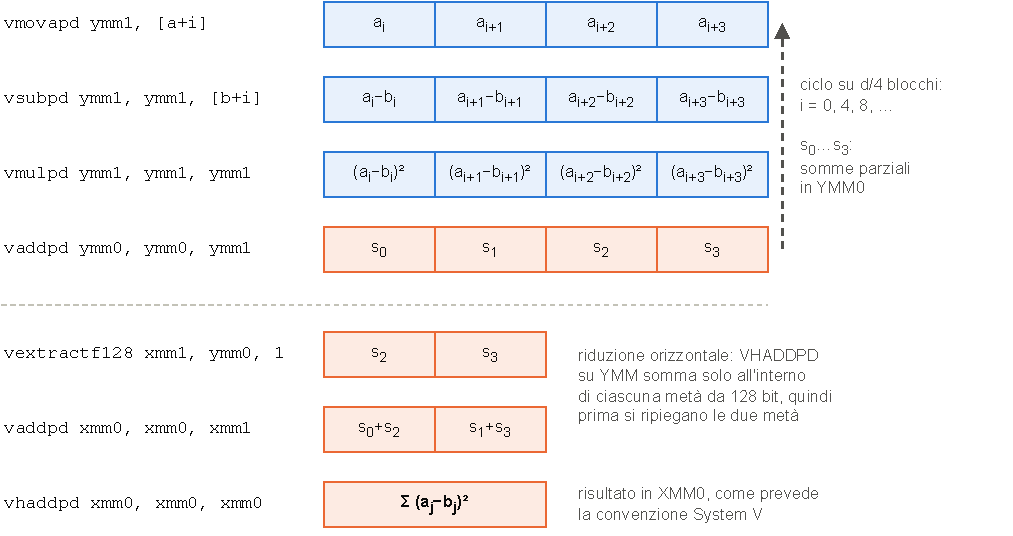
\includegraphics[width=\textwidth]{diagrammi/simd.pdf}
    \caption{Una iterazione del kernel AVX e la riduzione finale delle quattro somme parziali.}
    \label{fig:simd}
\end{figure}

La riduzione finale (Figura~\ref{fig:simd}) è diversa da quella a 32 bit perché \codice{vhaddpd} su registri YMM somma le coppie di valori all'interno di ciascuna metà da 128 bit, senza mai combinare le due metà: occorre prima estrarre la metà alta con \codice{vextractf128} e sommarla a quella bassa. Prima di tornare al chiamante, \codice{vzeroupper} azzera la metà alta dei registri YMM. Sui processori Intel~\cite{intel}, eseguire istruzioni SSE non codificate VEX mentre le metà alte sono \enquote{sporche} comporta una penalità di transizione, e il codice C compilato da GCC nel chiamante può contenerne. Per lo stesso motivo il kernel usa solo istruzioni con codifica VEX, mentre il kernel d'esame alternava istruzioni AVX e SSE (\codice{movsd}, \codice{subsd}, \codice{sqrtsd}) nello stesso ciclo e non eseguiva \codice{vzeroupper}.

Anche qui il kernel usa solo registri che la convenzione non chiede di preservare. Il kernel d'esame salvava invece quattro registri con \codice{push rax, rbx, rcx, rdi} e li ripristinava con \codice{pop} nello stesso ordine, anziché in ordine inverso: al ritorno \codice{RBX}, che il chiamante si aspetta invariato, conteneva il valore di \codice{RCX}. Il programma funzionava solo perché il codice generato con \codice{-O0} non usava \codice{RBX} in quel punto. Nella stessa versione, la macro \codice{popaq} fornita con il template ripristinava anche i registri YMM, sovrascrivendo il risultato appena calcolato in \codice{XMM0}: è questo il comportamento osservato nella relazione d'esame e attribuito, erroneamente, al processore.

\section{Il Riempimento delle Etichette}

\codice{fill\_labels\_simd} replica un intero in tutte le corsie di un registro e lo scrive a blocchi: quattro etichette per istruzione con SSE (\codice{pshufd} e \codice{movdqa}), otto con AVX. L'estensione AVX non dispone di rimescolamenti su interi a 256 bit, quindi il valore viene replicato in un registro XMM e copiato nella metà alta con \codice{vinsertf128}. Un breve ciclo scalare scrive le etichette residue quando $n$ non è multiplo della larghezza del registro. Rispetto alla versione d'esame, il valore da scrivere è un parametro invece di una costante in memoria, e le condizioni di uscita sono corrette per ogni $n$, compresi i valori minori di quattro.

\section{Confronto con il Codice del Compilatore}
\label{sec:compilatore}

Il template del corso prescriveva la compilazione con \codice{-O0}, per rendere evidente il contributo del codice assembly. La versione attuale è compilata con \codice{-O2}, e a questo livello GCC vettorizza da sé il ciclo della versione C del kernel. Il codice generato (Listato~\ref{lst:gcc}) mostra però che la vettorizzazione è solo parziale.

\begin{lstlisting}[language=nasm, caption={Ciclo di \codice{dist2\_c} generato da GCC 16 con \codice{-O2 -mavx} (sintassi AT\&T).}, label={lst:gcc}]
.L4:    vmovupd     (%rdi,%rax), %ymm1
        vsubpd      (%rsi,%rax), %ymm1, %ymm1
        addq        $32, %rax
        vmulpd      %ymm1, %ymm1, %ymm1
        vaddsd      %xmm1, %xmm0, %xmm0
        vunpckhpd   %xmm1, %xmm1, %xmm2
        vextractf128 $0x1, %ymm1, %xmm1
        vaddsd      %xmm2, %xmm0, %xmm0
        vaddsd      %xmm1, %xmm0, %xmm0
        vunpckhpd   %xmm1, %xmm1, %xmm1
        vaddsd      %xmm1, %xmm0, %xmm0
        cmpq        %rcx, %rax
        jne         .L4
\end{lstlisting}

Sottrazioni e quadrati sono calcolati quattro alla volta, ma i quadrati vengono poi sommati all'accumulatore uno per volta, in ordine, con quattro \codice{vaddsd} dipendenti l'una dall'altra. La somma in virgola mobile non è associativa, e senza un permesso esplicito (\codice{-ffast-math} o \codice{-fassociative-math}) il compilatore non può cambiare l'ordine delle addizioni. Il kernel scritto a mano lo cambia deliberatamente, mantenendo quattro somme parziali indipendenti, e completa un'iterazione con una sola somma vettoriale invece di una catena di quattro. Il risultato può differire da quello sequenziale nelle ultime cifre, ma i test del Capitolo~\ref{cap:sperimentazione} verificano che le etichette non cambiano. La Sezione~\ref{sec:esp-compilatore} misura il vantaggio che resta al codice scritto a mano con entrambi i livelli di ottimizzazione.

\chapter{Parallelizzazione con OpenMP}
\label{cap:openmp}

\section{L'Approccio della Versione d'Esame}

OpenMP~\cite{openmp} permette di parallelizzare un programma C annotandolo con direttive \codice{\#pragma omp}, che il compilatore traduce in codice multi-thread quando si compila con l'opzione \codice{-fopenmp}. La versione d'esame manteneva l'algoritmo originale, con le interrogazioni intrecciate all'espansione, e cercava il parallelismo all'interno della singola interrogazione:

\begin{itemize}
    \item la visita ricorsiva del Ball Tree apriva una regione \codice{parallel sections} per esplorare in parallelo i due figli di ogni nodo;
    \item la scansione di una foglia era un ciclo \codice{parallel for}, con una sezione \codice{critical} attorno a ogni inserimento di un punto nel risultato;
    \item l'assegnazione dell'etichetta ai punti di un intorno era a sua volta un ciclo \codice{parallel for}.
\end{itemize}

L'approccio aveva tre problemi. Il primo è che non è mai stato eseguito: gli script di compilazione della cartella OpenMP non passavano l'opzione \codice{-fopenmp}, il compilatore ignorava le direttive, e il binario a 32 bit \enquote{con OpenMP} risultava identico byte per byte a quello senza. Il secondo è la granularità: una interrogazione dura pochi microsecondi, meno del costo di creare e sincronizzare un gruppo di thread, e ogni livello della ricorsione ne apriva uno nuovo; la sezione critica serializzava poi proprio gli inserimenti. Il terzo è la misura: il tempo era calcolato con \codice{clock()}, che restituisce il tempo di CPU del processo, cioè la somma dei tempi di tutti i thread, e che con più thread cresce anche quando il programma diventa più veloce. La relazione d'esame dichiarava infatti di non poter misurare il beneficio di OpenMP.

\section{Parallelizzazione della Prima Fase}

La formulazione in due fasi (Sezione~\ref{sec:due-fasi}) sposta il parallelismo al livello più alto possibile: le $n$ interrogazioni della prima fase sono indipendenti e vengono distribuite tra i thread con un unico ciclo parallelo (Figura~\ref{fig:fasi}).

\begin{lstlisting}[language=C, caption={La prima fase in \codice{src/dbscan.c}, semplificata.}, label={lst:fase1}]
#pragma omp parallel reduction(+ : evals, kept, core_points)
{
    PointList found; // riusata da tutte le interrogazioni del thread
    point_list_init(&found, 256);
#pragma omp for schedule(dynamic, 64)
    for (int p = 0; p < n; p++) {
        point_list_clear(&found);
        evals += ball_tree_query(&tree, ds, p, eps, dist2, &found);
        is_core[p] = found.size + 1 >= min_pts;
        if (is_core[p])
            neighbours[p] = copia di found.items;
    }
    point_list_free(&found);
}
\end{lstlisting}

\begin{figure}[H]
    \centering
    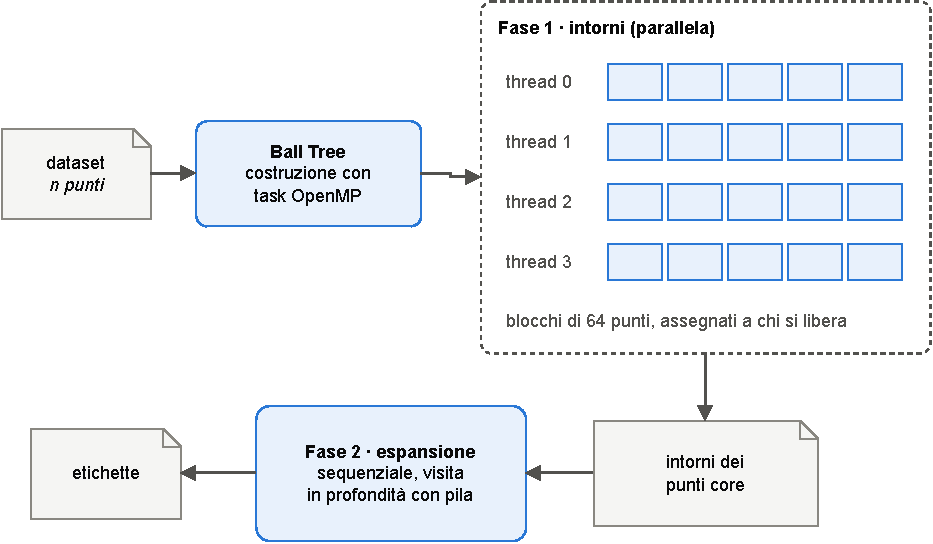
\includegraphics[width=\textwidth]{diagrammi/fasi.pdf}
    \caption{Le due fasi dell'algoritmo: la costruzione del Ball Tree e le interrogazioni sono parallele, l'espansione dei cluster è sequenziale.}
    \label{fig:fasi}
\end{figure}

Le scelte principali sono tre:

\begin{itemize}
    \item \textbf{nessuna sincronizzazione nel ciclo}: ogni iterazione scrive solo nelle celle di indice $p$ dei vettori \codice{is\_core}, \codice{count} e \codice{neighbours}, e ogni thread ha la propria lista temporanea. I contatori statistici sono sommati con una clausola \codice{reduction};
    \item \textbf{assegnazione dinamica}: il costo di un'interrogazione varia molto da punto a punto, perché un punto al centro di un cluster ha molti vicini e un punto isolato quasi nessuno. Con \codice{schedule(dynamic, 64)} i thread prelevano blocchi di 64 punti man mano che si liberano, invece di ricevere in anticipo una porzione fissa, e il carico si bilancia da sé. Il blocco di 64 punti rende trascurabile il costo della distribuzione;
    \item \textbf{ordine indipendente dai thread}: ogni intorno contiene sempre gli stessi punti, e la seconda fase li legge in ordine di indice. Il risultato è quindi identico con qualunque numero di thread, come verificano i test.
\end{itemize}

\section{Costruzione Parallela del Ball Tree}

La costruzione del Ball Tree è ricorsiva e i due sottoalberi di un nodo sono indipendenti, perché occupano intervalli disgiunti del vettore \codice{order}. Ogni chiamata ricorsiva diventa quindi un \emph{task} OpenMP, creato all'interno di una regione parallela da un solo thread (\codice{single}) ed eseguito da un thread qualunque del gruppo; \codice{taskwait} attende i due figli prima di restituire il nodo. Sotto i 4096 punti la clausola \codice{if} esegue il sottoalbero direttamente, perché un task così piccolo costerebbe più di quanto fa risparmiare. Il guadagno è limitato dal fatto che la suddivisione della radice, che esamina tutti i punti, è necessariamente eseguita da un solo thread; la costruzione pesa comunque circa l'1\% del tempo totale.

\section{Perché l'Espansione Resta Sequenziale}

La seconda fase non calcola distanze: visita un grafo i cui archi sono già noti, con un costo proporzionale alla somma delle dimensioni degli intorni. Nelle misure pesa tra lo 0,2\% e l'1\% del tempo totale, secondo il numero di thread, quindi parallelizzarla porterebbe un beneficio trascurabile. Sarebbe anche difficile farlo senza cambiare il risultato: due thread che espandono cluster diversi possono contendersi un punto di confine, e l'assegnazione al primo cluster che lo raggiunge richiede un ordine di visita definito. Una versione parallela dovrebbe calcolare le componenti connesse dei punti core con una struttura \emph{union-find} e assegnare i punti di confine in un passo successivo (Capitolo~\ref{cap:limiti}).

\section{Misura del Tempo}

Il programma misura il tempo reale trascorso, con la funzione \codice{clock\_gettime} e l'orologio monotono del sistema, separatamente per la costruzione dell'indice, la prima e la seconda fase. Il tempo riportato comprende solo il clustering e non la lettura del file, come nella versione d'esame, così che le due siano confrontabili. Per la versione d'esame, che è sequenziale, il tempo di CPU misurato da \codice{clock()} coincide in pratica con il tempo reale.

\chapter{Validazione e Analisi Sperimentale}
\label{cap:sperimentazione}

\section{Ambiente e Metodologia}

Tutte le misure sono state eseguite sulla macchina descritta nella Tabella~\ref{tab:ambiente} e sono riproducibili con \codice{make bench}, che genera i dataset, esegue gli esperimenti e salva i risultati grezzi nella cartella \codice{results}; lo script \codice{report\_data.py} ne ricava le tabelle e i grafici di questo capitolo.

\begin{table}[H]
    \centering
    \small
    \begin{tabularx}{\textwidth}{lX}
        \toprule
        \tabella{ambiente}
        \bottomrule
    \end{tabularx}
    \caption{Ambiente delle misure.}
    \label{tab:ambiente}
\end{table}

\subsection*{Dataset}

Salvo dove indicato, i dataset sono generati con la funzione \codice{make\_blobs} di scikit-learn: otto cluster gaussiani con deviazione standard unitaria, a cui si aggiunge un 5\% di punti distribuiti uniformemente nel riquadro che li contiene, a fare da rumore. \textit{MinPts} vale 5 e $\varepsilon$ è scelto con l'euristica del lavoro originale~\cite{ester1996}, basata sulla distanza di ogni punto dal suo quarto vicino: si prende il valore che lascia il 90\% dei punti al di sotto, così che circa il 90\% dei punti sia core. Il dataset usato per l'esame, invece, contiene 5000 punti distribuiti uniformemente nell'ipercubo unitario a 50 dimensioni, con $\varepsilon = 5$.

\subsection*{Misure}

Ogni valore è la mediana di cinque esecuzioni. Il tempo è quello misurato dal programma per il solo clustering, dalla costruzione dell'indice alla fine dell'espansione, con la lettura del file esclusa; per scikit-learn è il tempo della chiamata a \codice{fit}. La macchina è un portatile, con frequenza del processore variabile in base al carico e alla temperatura: le misure ripetute differiscono tipicamente di qualche punto percentuale, e minimo e massimo di ogni serie sono riportati nei file dei risultati.

\section{Correttezza}

Lo script \codice{tests/run\_tests.py}, eseguito da \codice{make test} e dall'integrazione continua a ogni modifica, confronta le etichette prodotte da ogni eseguibile con quelle di scikit-learn su nove casi:

\begin{itemize}
    \item tre dataset con cluster in 2, 13 e 64 dimensioni, di cui la seconda non multipla di quattro, per verificare il padding;
    \item il dataset uniforme dell'esame con $\varepsilon = 5$, un unico cluster, e con $\varepsilon = 1{,}2$, tutto rumore;
    \item 300 punti identici, il caso che nella versione d'esame causava la ricorsione infinita;
    \item $\textit{MinPts} = 1$, in cui ogni punto è core;
    \item dataset di uno e di tre punti, più piccoli di un registro SIMD.
\end{itemize}

Ogni caso è eseguito con la ricerca esaustiva e con il Ball Tree, con foglie da 1 e da 32 punti, con i kernel SIMD e con quelli in C, e per le varianti OpenMP con 1 e con 4 thread. Per le varianti a 64 bit le etichette devono coincidere con quelle di scikit-learn punto per punto, e coincidono in tutti i casi; per le varianti a 32 bit, che lavorano in singola precisione, è ammessa una differenza fino allo 0,2\% dei punti, per i motivi discussi nel Capitolo~\ref{cap:limiti}, ma nei casi di prova le etichette coincidono esattamente anche a 32 bit. Lo script verifica anche la gestione degli errori della riga di comando. Il programma è stato inoltre eseguito con Valgrind, senza errori di accesso alla memoria né memoria non liberata, e compilato con l'\emph{Undefined Behavior Sanitizer} di GCC, senza segnalazioni.

\section{Confronto tra le Varianti}
\label{sec:varianti}

La Tabella~\ref{tab:varianti-blobs} e la Figura~\ref{fig:varianti} confrontano le varianti del programma sul dataset di 20.000 punti in 16 dimensioni, aggiungendo un'ottimizzazione alla volta, insieme alla versione d'esame e a scikit-learn.

\begin{table}[H]
    \centering
    \small
    \begin{tabular}{lrrr}
        \toprule
        \textbf{Variante} & \textbf{Tempo (s)} & \textbf{Speedup} & \textbf{Distanze calcolate} \\
        \midrule
        \tabella{varianti_blobs}
        \bottomrule
    \end{tabular}
    \caption{Varianti a confronto su 20.000 punti in 16 dimensioni; lo speedup è rispetto alla versione d'esame.}
    \label{tab:varianti-blobs}
\end{table}

\begin{figure}[H]
    \centering
    % Tempo di ogni variante sul dataset di 20.000 punti (dati/varianti_blobs.csv)
\begin{tikzpicture}
\begin{axis}[
    relazione,
    xbar,
    width=0.72\textwidth,
    height=0.6\textwidth,
    bar width=8pt,
    xmin=0,
    xmax=3.9,
    enlarge y limits=0.07,
    xlabel={Tempo di esecuzione (s)},
    ytick=data,
    yticklabels from table={\dati{varianti_blobs}}{variante},
    table/col sep=semicolon,
    y tick label style={font=\footnotesize, color=inchiostro},
    ymajorgrids=false,
    nodes near coords,
    nodes near coords style={font=\footnotesize, color=inchiostro,
        /pgf/number format/.cd, fixed, fixed zerofill, precision=2, use comma},
]
\addplot[fill=serie1, draw=none] table[col sep=semicolon, x=tempo, y expr=\coordindex]{\dati{varianti_blobs}};
\end{axis}
\end{tikzpicture}

    \caption{Tempo di esecuzione delle varianti su 20.000 punti in 16 dimensioni.}
    \label{fig:varianti}
\end{figure}

La lettura della tabella dall'alto verso il basso mostra il contributo di ciascuna tecnica:

\begin{itemize}
    \item \textbf{Kernel SIMD.} A parità di algoritmo, i kernel AVX riducono il tempo di 1,7 volte con la ricerca esaustiva e di 1,4 volte con il Ball Tree, dove una parte del tempo va nella visita dell'albero e non nel calcolo delle distanze.
    \item \textbf{Ball Tree.} L'indice calcola sei volte meno distanze della ricerca esaustiva e riduce il tempo di quattro volte. Da solo, anche senza SIMD, porta il programma a quasi tre volte la velocità della versione d'esame.
    \item \textbf{OpenMP.} Con quattro thread, uno per core fisico, il tempo si riduce di 3,3 volte; con otto thread di 3,8 volte. Il programma completo è 16 volte più veloce della versione d'esame.
    \item \textbf{Confronto con scikit-learn.} Su un solo thread il programma è più lento di scikit-learn del 34\%. scikit-learn con tutti i thread (\codice{n\_jobs=-1}) migliora di poco, perché la sua espansione dei cluster è sequenziale e le interrogazioni sono parallelizzate solo in parte. Con otto thread il programma è 2,8 volte più veloce.
\end{itemize}

La versione d'esame, compilata con \codice{-O0} come prescritto dal corso, impiega poco più della ricerca esaustiva con i kernel AVX, benché usi un Ball Tree: le foglie da 300 punti e le numerose allocazioni ne annullano quasi del tutto il vantaggio.

\section{Confronto tra 32 e 64 Bit}

La Tabella~\ref{tab:architetture} confronta le due architetture sullo stesso dataset: a sinistra la variante a 32 bit, con kernel SSE in singola precisione, a destra quella a 64 bit, con kernel AVX in doppia precisione. L'ultima colonna è il rapporto tra i tempi: un valore minore di uno indica che la variante a 64 bit è più veloce.

\begin{table}[H]
    \centering
    \small
    \begin{tabular}{lrrr}
        \toprule
        \textbf{Variante} & \textbf{32 bit, SSE (s)} & \textbf{64 bit, AVX (s)} & \textbf{Rapporto} \\
        \midrule
        \tabella{architetture}
        \bottomrule
    \end{tabular}
    \caption{Variante a 32 bit e variante a 64 bit su 20.000 punti in 16 dimensioni.}
    \label{tab:architetture}
\end{table}

La variante a 64 bit richiede dal 14 al 27\% di tempo in meno in tutti i casi, benché lavori in doppia precisione e quindi con il doppio dei dati. Le due varianti elaborano lo stesso numero di valori per istruzione, quattro \codice{float} in un registro XMM o quattro \codice{double} in un registro YMM, e la singola precisione non porta quindi alcun vantaggio nel calcolo. Pesano invece due caratteristiche della modalità a 32 bit:

\begin{itemize}
    \item la convenzione \emph{cdecl} passa gli argomenti sullo stack e restituisce il risultato sullo stack x87, che il codice compilato con \codice{-mfpmath=sse} deve poi riportare in un registro XMM passando per la memoria: ogni distanza attraversa la memoria due volte, nel kernel (\codice{movss} e \codice{fld}) e nel chiamante (\codice{fstp} e \codice{movss});
    \item l'architettura a 32 bit dispone di 8 registri generali e 8 registri XMM, contro 16 e 16, e il compilatore deve salvare in memoria più variabili, come mostra il rallentamento anche delle varianti in C.
\end{itemize}

Una variante a 32 bit che usasse AVX in singola precisione elaborerebbe otto valori per istruzione, ma il corso prescriveva le sole istruzioni SSE per questa architettura.

\section{Il Caso della Versione d'Esame}
\label{sec:caso-esame}

La relazione d'esame osservava che il Ball Tree non portava miglioramenti significativi rispetto alla ricerca esaustiva, e ne attribuiva la causa al costo di costruzione, alla dimensione delle foglie e allo sbilanciamento dell'albero. La causa principale era in realtà il dataset. In un ipercubo unitario a 50 dimensioni la distanza tra due punti casuali si concentra attorno a $\sqrt{50/6} \approx 2{,}9$: nel dataset dell'esame la media è 2,88, la deviazione standard 0,24 e la distanza massima 4,16. Con $\varepsilon = 5$ ogni punto ha quindi per vicini tutti gli altri, e il risultato è un unico cluster. Nessuna sfera dell'albero può essere disgiunta dall'intorno, e un indice che sa solo escludere le regioni lontane non può escludere nulla.

\begin{table}[H]
    \centering
    \small
    \begin{tabular}{lrrr}
        \toprule
        \textbf{Variante} & \textbf{Tempo (s)} & \textbf{Speedup} & \textbf{Distanze calcolate} \\
        \midrule
        \tabella{varianti_esame}
        \bottomrule
    \end{tabular}
    \caption{Varianti a confronto sul dataset dell'esame: 5000 punti uniformi in 50 dimensioni, $\varepsilon = 5$.}
    \label{tab:varianti-esame}
\end{table}

La Tabella~\ref{tab:varianti-esame} mostra l'effetto dell'accettazione in blocco delle sfere interamente contenute nell'intorno: per quasi ogni interrogazione la sfera della radice cade tutta dentro l'intorno, e il Ball Tree calcola 5053 distanze invece di 25 milioni. Il tempo che resta è speso quasi tutto nel copiare gli intorni, 25 milioni di indici e 100~MB di memoria, ed è per questo che i kernel SIMD non vi incidono. Con la ricerca esaustiva, invece, il vantaggio dei kernel AVX sale a 2,3 volte, perché con 52 valori per riga ogni chiamata del kernel esegue 13 iterazioni e il costo fisso della chiamata pesa meno.

Il caso è istruttivo anche per un altro motivo: un dataset in cui tutti i punti formano un solo cluster non può rivelare errori nell'assegnazione delle etichette. Per questo i test e le misure di questo capitolo usano dataset con cluster reali e rumore, e il dataset dell'esame compare solo come caso limite.

\section{Scalabilità con i Thread}

La Figura~\ref{fig:threads} riporta lo speedup della prima fase parallela rispetto all'esecuzione su un thread, per il Ball Tree su 80.000 punti e per la ricerca esaustiva su 20.000 punti, entrambi in 16 dimensioni.

\begin{figure}[H]
    \centering
    % Speedup rispetto a un thread (dati/threads.csv)
\begin{tikzpicture}
\begin{axis}[
    relazione,
    xmin=1, xmax=8, ymin=0, ymax=8.5,
    xtick={1,...,8},
    xlabel={Thread OpenMP},
    ylabel={Speedup rispetto a 1 thread},
    legend pos=north west,
]
\addplot[muto, dashed, line width=0.8pt, forget plot] table[col sep=comma, x=threads, y=ideale]{\dati{threads}}
    node[pos=0.93, above left, font=\footnotesize, text=muto] {ideale};
\draw[muto, dotted, line width=0.8pt] (axis cs:4,0) -- (axis cs:4,8.5)
    node[pos=0.97, right, font=\footnotesize, text=muto] {4 core fisici};
\addplot[serie1, mark=*] table[col sep=comma, x=threads, y=balltree]{\dati{threads}};
\addlegendentry{Ball Tree, 80.000 punti}
\addplot[serie2, mark=square*] table[col sep=comma, x=threads, y=linear]{\dati{threads}};
\addlegendentry{Ricerca esaustiva, 20.000 punti}
\end{axis}
\end{tikzpicture}

    \caption{Speedup al crescere dei thread OpenMP. La linea tratteggiata è lo speedup ideale, la linea punteggiata il numero di core fisici.}
    \label{fig:threads}
\end{figure}

Fino a quattro thread, uno per core fisico, lo speedup è di 3,0 per il Ball Tree e di 3,3 per la ricerca esaustiva. Non raggiunge il valore ideale per due motivi. Il primo è la frequenza del processore, che con un solo core attivo sale fino a 4~GHz e scende quando lavorano tutti i core. Il secondo, per il Ball Tree, è l'accesso alla memoria meno regolare della visita dell'albero, con i core in competizione per la cache condivisa. Oltre quattro thread l'\emph{hyper-threading} esegue due thread sullo stesso core fisico e aggiunge un altro 20--25\%, fino a 3,8 e 3,9 con otto thread: i due thread di un core si alternano sulle stesse unità di calcolo e ne coprono i tempi di attesa.

La parte sequenziale è trascurabile: l'espansione dei cluster richiede circa 20~ms su 80.000 punti, lo 0,2\% del tempo su un thread e l'1\% su otto, e la costruzione del Ball Tree passa da 104 a 72~ms. Secondo la legge di Amdahl, una parte sequenziale pari all'1\% del tempo pone allo speedup un limite teorico di 100.

\section{Scalabilità con il Numero di Punti}

La Figura~\ref{fig:scaling} riporta il tempo di esecuzione al crescere del numero di punti da 5000 a 80.000, in 16 dimensioni e in scala logaritmica su entrambi gli assi, dove una retta di pendenza 2 indica un costo quadratico. La ricerca esaustiva si ferma a 40.000 punti, perché con 80.000 richiederebbe circa 40 secondi per esecuzione.

\begin{figure}[H]
    \centering
    % Tempo al crescere del numero di punti, d = 16 (dati/scaling.csv)
\begin{tikzpicture}
\begin{loglogaxis}[
    relazione,
    xlabel={Numero di punti $n$},
    ylabel={Tempo di esecuzione (s)},
    xtick={5000,10000,20000,40000,80000},
    xticklabels={5.000,10.000,20.000,40.000,80.000},
    legend pos=north west,
    unbounded coords=discard,
]
\addplot[serie2, mark=square*] table[col sep=comma, x=n, y=linear]{\dati{scaling}};
\addlegendentry{Ricerca esaustiva, AVX}
\addplot[serie1, mark=*] table[col sep=comma, x=n, y=balltree]{\dati{scaling}};
\addlegendentry{Ball Tree, AVX}
\addplot[serie3, mark=triangle*, mark size=3pt] table[col sep=comma, x=n, y=omp8]{\dati{scaling}};
\addlegendentry{Ball Tree, AVX, 8 thread}
\addplot[inchiostro, dashed, mark=o] table[col sep=comma, x=n, y=sklearn]{\dati{scaling}};
\addlegendentry{scikit-learn, 1 thread}
\end{loglogaxis}
\end{tikzpicture}

    \caption{Tempo di esecuzione al crescere del numero di punti, in 16 dimensioni.}
    \label{fig:scaling}
\end{figure}

Tutte le curve hanno pendenza vicina a 2, compresa quella di scikit-learn: raddoppiando i punti il tempo quadruplica anche con il Ball Tree, e il numero di distanze calcolate passa da 4,3 milioni a un miliardo. Non è un difetto dell'indice ma una proprietà dei dati: con un numero fisso di cluster, raddoppiare i punti raddoppia la densità e quindi la dimensione media degli intorni, mentre $\varepsilon$ scelto con l'euristica diminuisce di poco. La dimensione complessiva del risultato cresce quindi in modo quadratico, e nessun algoritmo che elenchi gli intorni può fare meglio, come osservano Schubert et al.~\cite{schubert2017}. Il Ball Tree abbassa la costante, di un fattore compreso tra 3,5 e 5 rispetto alla ricerca esaustiva, e OpenMP la abbassa di un ulteriore fattore compreso tra 3 e 4.

\section{Dimensione delle Foglie}

Il parametro \textit{leaf\_size} regola un compromesso: foglie piccole producono un albero profondo, con più nodi da visitare e più distanze dai centri da calcolare; foglie grandi producono un albero basso ma costringono a esaminare molti punti lontani in ogni foglia raggiunta. La Figura~\ref{fig:foglie} riporta il tempo in funzione della dimensione delle foglie, diviso per il tempo migliore di ciascun dataset.

\begin{figure}[H]
    \centering
    % Tempo relativo al migliore al variare della dimensione delle foglie (dati/leaf_size.csv)
\begin{tikzpicture}
\begin{semilogxaxis}[
    relazione,
    log basis x=2,
    xtick={1,4,16,64,256,1024},
    xticklabels={1,4,16,64,256,1024},
    xlabel={Punti massimi per foglia (\textit{leaf\_size})},
    ylabel={Tempo relativo al migliore},
    ymin=0.9,
    legend pos=north west,
]
\addplot[serie1, mark=*] table[col sep=comma, x=leaf, y=d2]{\dati{leaf_size}};
\addlegendentry{$n = 20.000$, $d = 2$}
\addplot[serie2, mark=square*] table[col sep=comma, x=leaf, y=d16]{\dati{leaf_size}};
\addlegendentry{$n = 40.000$, $d = 16$}
\addplot[serie3, mark=triangle*, mark size=3pt] table[col sep=comma, x=leaf, y=d64]{\dati{leaf_size}};
\addlegendentry{$n = 20.000$, $d = 64$}
\end{semilogxaxis}
\end{tikzpicture}

    \caption{Tempo al variare della dimensione massima delle foglie, relativo al valore migliore di ciascun dataset.}
    \label{fig:foglie}
\end{figure}

Il valore migliore dipende dalla dimensionalità: 16 punti in due dimensioni, 128 in 16 e in 64 dimensioni. In poche dimensioni le sfere sono piccole e ben separate, e conviene scendere in profondità per escluderne di più; in molte dimensioni la potatura è comunque limitata e conviene ridurre il costo della visita. Il valore predefinito, 32, resta entro l'8\% dal migliore in tutti e tre i casi, mentre sia 128 sia valori molto piccoli penalizzano uno dei casi di oltre il 40\%. Le 300 foglie della versione d'esame erano un valore ragionevole in molte dimensioni, ma avrebbero raddoppiato il tempo nel caso bidimensionale.

\section{Effetto della Dimensionalità}
\label{sec:esp-dimensioni}

La Tabella~\ref{tab:dimensioni} e la Figura~\ref{fig:dimensioni} confrontano il Ball Tree con la ricerca esaustiva su 20.000 punti al variare della dimensione, da 2 a 128.

\begin{table}[H]
    \centering
    \small
    \begin{tabular}{rrrrrr}
        \toprule
        $d$ & \textbf{Esaustiva (s)} & \textbf{Ball Tree (s)} & \textbf{Speedup} & \textbf{Distanze} & \textbf{Profondità} \\
        \midrule
        \tabella{dimensioni}
        \bottomrule
    \end{tabular}
    \caption{Ball Tree e ricerca esaustiva al variare della dimensione, su 20.000 punti; la colonna Distanze riporta le distanze calcolate dal Ball Tree in percentuale di quelle della ricerca esaustiva.}
    \label{tab:dimensioni}
\end{table}

\begin{figure}[H]
    \centering
    % Distanze calcolate dal Ball Tree rispetto alla ricerca esaustiva (dati/dimensions.csv)
\begin{tikzpicture}
\begin{semilogxaxis}[
    relazione,
    height=0.55\textwidth,
    log basis x=2,
    xtick={2,4,8,16,32,64,128},
    xticklabels={2,4,8,16,32,64,128},
    xlabel={Dimensioni $d$},
    ylabel={Distanze calcolate (\%)},
    ymin=0,
    nodes near coords,
    nodes near coords style={font=\footnotesize, color=inchiostro, anchor=south,
        /pgf/number format/.cd, fixed, precision=1, use comma},
]
\addplot[serie1, mark=*] table[col sep=comma, x=d, y=percentuale]{\dati{dimensions}};
\end{semilogxaxis}
\end{tikzpicture}

    \caption{Distanze calcolate dal Ball Tree, in percentuale di quelle della ricerca esaustiva, al variare della dimensione.}
    \label{fig:dimensioni}
\end{figure}

In due dimensioni il Ball Tree calcola l'1,3\% delle distanze ed è 21 volte più veloce della ricerca esaustiva. La percentuale cresce con la dimensione, com'è tipico degli indici spaziali: in molte dimensioni le distanze tendono a somigliarsi e le sfere si sovrappongono. La crescita però si arresta attorno al 20\% invece di proseguire fino al 100\%. Il motivo sta nella struttura dei dati: gli otto cluster restano ben separati in qualunque dimensione, e l'albero continua a escludere in blocco i cluster diversi da quello del punto interrogato, anche quando all'interno di un cluster non riesce più a potare. Con otto cluster di dimensioni simili resta da esaminare circa un ottavo dei punti, più il rumore e i nodi a cavallo di due cluster. Su dati senza alcuna struttura, come il dataset uniforme dell'esame con un $\varepsilon$ più piccolo, la potatura in alta dimensione sarebbe molto minore.

\section{SIMD Manuale e Ottimizzazioni del Compilatore}
\label{sec:esp-compilatore}

La Tabella~\ref{tab:compilatore} confronta i kernel in C e quelli SIMD con i due livelli di ottimizzazione: \codice{-O0}, prescritto dal template del corso, e \codice{-O2}, usato dalla versione attuale.

\begin{table}[H]
    \centering
    \small
    \begin{tabular}{llrrr}
        \toprule
        \textbf{Indice} & \textbf{Livello} & \textbf{C (s)} & \textbf{SIMD (s)} & \textbf{Vantaggio} \\
        \midrule
        \tabella{compilatore}
        \bottomrule
    \end{tabular}
    \caption{Kernel in C e kernel SIMD con i livelli di ottimizzazione \codice{-O0} e \codice{-O2}, su 20.000 punti in 16 dimensioni.}
    \label{tab:compilatore}
\end{table}

Con \codice{-O0} i kernel SIMD sembrano da 4,3 a 5,6 volte più veloci, ma il confronto è sbilanciato: senza ottimizzazioni il compilatore rilegge e riscrive in memoria ogni variabile a ogni iterazione, e la versione in C è molto più lenta del necessario. Con \codice{-O2} il vantaggio scende a 1,5--1,7 volte, ed è il valore che misura davvero il contributo del codice scritto a mano: nasce dalle quattro somme parziali indipendenti che il compilatore non può introdurre da sé (Sezione~\ref{sec:compilatore}). Anche il resto del programma beneficia delle ottimizzazioni: la visita del Ball Tree e la gestione delle liste, che non usano i kernel, fanno scendere del 40\% il tempo del Ball Tree con i kernel SIMD tra \codice{-O0} e \codice{-O2}.

\chapter{Limiti e Sviluppi Possibili}
\label{cap:limiti}

\section{Memoria Occupata dagli Intorni}

Il limite principale della formulazione in due fasi è la memoria: gli intorni dei punti core restano in memoria fino all'espansione, per un totale di quattro byte per ogni coppia di punti vicini. Sui dataset con cluster ben definiti usati nelle prove il costo è contenuto, ma quando $\varepsilon$ è grande rispetto alla scala dei dati gli intorni diventano enormi: sul dataset uniforme dell'esame ogni punto ha per vicini tutti gli altri, e 5000 punti richiedono già 100~MB. Con 50.000 punti ne servirebbero 10~GB. scikit-learn condivide lo stesso limite, perché calcola tutti gli intorni in anticipo.

Due varianti ridurrebbero la memoria senza rinunciare al parallelismo:

\begin{itemize}
    \item memorizzare solo gli archi tra punti core, più per ogni punto non core un solo punto core vicino, e calcolare le componenti connesse con una struttura \emph{union-find}; è l'approccio di diverse implementazioni parallele di DBSCAN e renderebbe parallela anche l'espansione;
    \item elaborare i punti a blocchi, calcolando e consumando gli intorni di un blocco alla volta, al prezzo di interrogare di nuovo i punti al confine tra blocchi.
\end{itemize}

\section{La Matrice delle Distanze}

La relazione d'esame proponeva di precalcolare la matrice di tutte le distanze, per non calcolare mai due volte la stessa. Nella formulazione attuale il problema non si pone, perché ogni coppia viene esaminata al più due volte, una per ciascun punto, e le interrogazioni del Ball Tree ne escludono la maggior parte; la matrice richiederebbe inoltre $n^2$ valori, 20~GB in doppia precisione per 50.000 punti. Sfruttare la simmetria, calcolando ogni coppia una sola volta, dimezzerebbe il lavoro della ricerca esaustiva, ma complicherebbe la distribuzione del lavoro tra i thread.

\section{Kernel SIMD}

Il kernel della distanza ha un'unica catena di somme vettoriali: ogni iterazione deve attendere il risultato di \codice{vaddpd} dell'iterazione precedente, con una latenza di quattro cicli sui processori della famiglia Skylake. Mantenere due o quattro accumulatori indipendenti, sommati alla fine, lascerebbe lavorare in parallelo le unità di calcolo e ridurrebbe il costo per dimensioni elevate; richiederebbe però di arrotondare la dimensione a un multiplo di otto o sedici valori. Altre estensioni offrirebbero ulteriori margini, a costo di restringere i processori supportati:

\begin{itemize}
    \item le istruzioni FMA (\emph{fused multiply-add}) fonderebbero moltiplicazione e somma in un'unica istruzione;
    \item AVX-512 raddoppierebbe il numero di valori per registro; il processore usato per le misure non la supporta.
\end{itemize}

Il costo di una chiamata al kernel, attraverso un puntatore a funzione, pesa infine sulle dimensioni piccole: con $d = 2$ una distanza richiede una sola iterazione del ciclo. Un kernel che confronti un punto con un'intera foglia in una sola chiamata ammortizzerebbe questo costo.

\section{Struttura dell'Indice}

Il Ball Tree riduce di molto le distanze calcolate in poche dimensioni, ma la sua efficacia cala al crescere della dimensione (Sezione~\ref{sec:esp-dimensioni}), come per ogni indice spaziale. scikit-learn sceglie automaticamente tra un \emph{k-d tree}, un Ball Tree e la ricerca esaustiva in base ai dati; una scelta analoga, insieme a una suddivisione dei nodi più accurata, per esempio lungo la direzione di massima varianza, migliorerebbe le prestazioni nei casi sfavorevoli. La relazione d'esame citava anche l'R-Tree, suggerito nel lavoro originale su DBSCAN, che è progettato per dati su disco e aggiornamenti dinamici, due esigenze assenti in questo contesto.

\section{Precisione della Variante a 32 Bit}

La variante a 32 bit lavora in singola precisione, come richiesto dal corso. Un punto la cui distanza da un vicino è pari a $\varepsilon$ entro l'errore di arrotondamento può cadere dalla parte opposta rispetto al calcolo in doppia precisione, e cambiare il proprio stato di punto core o di confine. Per questo i test accettano per la variante a 32 bit una piccola percentuale di etichette diverse da quelle di scikit-learn, mentre per quella a 64 bit richiedono l'uguaglianza esatta; nei dataset di prova, generati con valori casuali, il caso non si è mai presentato, ma su dati con coordinate ripetute o $\varepsilon$ pari a una distanza esistente non si può escludere.

\chapter{Conclusioni}

Il progetto ha realizzato DBSCAN in C e assembly x86 e lo ha accelerato combinando tre tecniche, ciascuna rivolta a un aspetto diverso del costo delle interrogazioni di vicinato. Sul dataset di riferimento, 20.000 punti in 16 dimensioni, il programma completo è sedici volte più veloce della versione consegnata all'esame e 2,8 volte più veloce di scikit-learn, producendo le stesse etichette punto per punto.

\section*{Il contributo di ciascuna tecnica}

\begin{itemize}
    \item \textbf{La struttura dati} è la leva più efficace: il Ball Tree riduce da tre a cinque volte il tempo rispetto alla ricerca esaustiva, e sui dati con $\varepsilon$ grande, grazie all'accettazione in blocco delle sfere, di diversi ordini di grandezza. Anche i dettagli di implementazione contano: la sola copia dei punti in ordine di foglia riduce il tempo del 20--40\%, un effetto paragonabile a quello dei kernel AVX, che con il Ball Tree lo riducono del 30\%.
    \item \textbf{Le istruzioni SIMD} riducono il costo di ogni distanza di 1,4--2,3 volte, di più quando le righe sono lunghe. Anche con \codice{-O2}, dove il compilatore vettorizza da sé, il codice scritto a mano conserva un vantaggio, perché può riordinare le somme in virgola mobile, cosa che al compilatore non è permessa.
    \item \textbf{OpenMP} porta uno speedup di 3 sui quattro core fisici e di quasi 4 con l'\emph{hyper-threading}, ma solo dopo aver riformulato l'algoritmo: il parallelismo va cercato al livello delle interrogazioni indipendenti e non all'interno della singola interrogazione, dove il costo della sincronizzazione supera il lavoro da distribuire.
\end{itemize}

\section*{Cosa ha insegnato la revisione}

La revisione della versione d'esame ha mostrato quanto una misura possa ingannare. OpenMP non era mai stato attivato e il tempo era misurato come tempo di CPU, quindi ogni considerazione sulla parallelizzazione era priva di riscontro. Il dataset di prova conteneva un solo cluster, quindi non poteva rivelare errori nelle etichette né mostrare i benefici dell'indice. Due errori nei kernel assembly, la violazione della convenzione di chiamata a 64 bit e la variabile globale condivisa a 32 bit, erano invisibili nelle condizioni in cui il programma veniva provato. Il confronto sistematico con un'implementazione di riferimento su casi tipici e limite, eseguito automaticamente a ogni modifica, è ciò che rende affidabili i risultati di questa versione.

\section*{Sviluppi futuri}

Gli sviluppi più promettenti, discussi nel Capitolo~\ref{cap:limiti}, sono tre:
\begin{itemize}
    \item ridurre la memoria occupata dagli intorni, e rendere parallela anche l'espansione, con una struttura \emph{union-find} sui punti core;
    \item usare più accumulatori nei kernel;
    \item scegliere l'indice spaziale in base alla dimensionalità dei dati.
\end{itemize}

\appendix
\chapter{Dalla Versione d'Esame alla Versione Attuale}
\label{app:modifiche}

La versione consegnata all'esame è conservata nel repository con l'etichetta \codice{exam-2024} e si può compilare con \codice{make exam}, che la costruisce come facevano gli script del corso. Questa appendice riassume le modifiche al template fornito dal docente e le differenze tra la versione d'esame e quella attuale.

\section{Modifiche al Template}

Il template del corso era stato pensato per un altro algoritmo e prevedeva un vettore di etichette in ingresso e un parametro \codice{k}, il numero di elementi da estrarre. Già nella versione d'esame erano stati aggiunti i parametri \textit{MinPts} ed $\varepsilon$ alla struttura dei parametri e alla riga di comando, con i relativi controlli, e la funzione di lettura era stata estesa per completare le righe del dataset a un multiplo di quattro valori (Sezione~\ref{sec:padding}). Il file delle etichette e il parametro \codice{k} erano però rimasti obbligatori, benché ignorati: il valore di \codice{k} veniva sovrascritto con il numero di punti. La versione attuale conserva il formato dei file del template ed elimina i parametri inutilizzati.

\section{Errori Corretti}

\begin{table}[H]
    \centering
    \small
    \begin{tabularx}{\textwidth}{XX}
        \toprule
        \textbf{Problema nella versione d'esame} & \textbf{Correzione} \\
        \midrule
        OpenMP mai attivato: mancava \codice{-fopenmp} negli script di compilazione &
        quattro varianti prodotte dal \codice{Makefile}, con e senza \codice{-fopenmp} \\
        Kernel a 64 bit: registri ripristinati in ordine errato, \codice{RBX} alterato &
        kernel che usano solo registri non da preservare \\
        Kernel a 32 bit: risultato restituito tramite una variabile globale, condivisa tra i thread &
        cella sullo stack del thread \\
        Tempo misurato con \codice{clock()}, cioè come tempo di CPU sommato su tutti i thread &
        tempo reale con \codice{clock\_gettime} \\
        File delle etichette con un elemento in più, letto oltre la fine del vettore &
        un'etichetta per punto \\
        Controllo dei limiti in \codice{getPuntiValue} con \codice{>} invece di \codice{>=}; estrazione da lista vuota non controllata &
        nuova \codice{PointList}, usata solo in modi che non richiedono controlli \\
        Ricorsione infinita nel Ball Tree con più di \codice{LEAFSIZE} punti identici &
        nodo foglia quando il raggio è nullo \\
        Memoria non liberata: albero, matrice originale dopo il padding, centroidi &
        ogni allocazione liberata; verificato con Valgrind \\
        Mix di istruzioni AVX e SSE senza \codice{vzeroupper} &
        solo istruzioni VEX e \codice{vzeroupper} all'uscita \\
        Intestazioni, nomi e messaggi ereditati da altri progetti (\codice{cfs}, \enquote{Attention mechanism}) &
        nomi e commenti riscritti \\
        \bottomrule
    \end{tabularx}
    \caption{Errori della versione d'esame e relative correzioni.}
    \label{tab:errori}
\end{table}

\section{Modifiche Strutturali}

\begin{itemize}
    \item \textbf{Un solo albero di sorgenti} al posto di quattro copie del programma, diviso in moduli e compilato da un \codice{Makefile}; commenti e identificatori in inglese.
    \item \textbf{Algoritmo in due fasi}, con la prima fase parallela e la regola di assegnazione dei punti di confine di scikit-learn.
    \item \textbf{Ball Tree} costruito per partizionamento sul posto, in parallelo, con i punti copiati in ordine di foglia e l'accettazione in blocco delle sfere interamente contenute nell'intorno.
    \item \textbf{Kernel SIMD} con interfaccia a puntatori, distanza al quadrato e uso anche per i centroidi.
    \item \textbf{Riga di comando} con opzioni per scegliere indice, kernel e numero di thread, e statistiche in formato JSON.
    \item \textbf{Verifica automatica}: script che confrontano le etichette con scikit-learn su casi tipici e limite, eseguiti anche dall'integrazione continua a ogni modifica, e script che riproducono tutte le misure di questa relazione.
\end{itemize}

\begin{thebibliography}{9}

\bibitem{ester1996}
M.~Ester, H.-P.~Kriegel, J.~Sander, X.~Xu,
\textit{A Density-Based Algorithm for Discovering Clusters in Large Spatial
Databases with Noise}, in Proceedings of the Second International Conference on
Knowledge Discovery and Data Mining (KDD~'96), AAAI Press, Portland, 1996,
pp.~226--231.

\bibitem{schubert2017}
E.~Schubert, J.~Sander, M.~Ester, H.-P.~Kriegel, X.~Xu,
\textit{DBSCAN Revisited, Revisited: Why and How You Should (Still) Use DBSCAN},
ACM Transactions on Database Systems, vol.~42, n.~3, 2017, art.~19.
\newblock DOI: \texttt{10.1145/3068335}.

\bibitem{omohundro1989}
S.~M.~Omohundro,
\textit{Five Balltree Construction Algorithms}, Technical Report TR-89-063,
International Computer Science Institute, Berkeley, 1989.

\bibitem{sklearn}
F.~Pedregosa, G.~Varoquaux, A.~Gramfort, V.~Michel, B.~Thirion, O.~Grisel,
M.~Blondel, P.~Prettenhofer, R.~Weiss, V.~Dubourg, J.~Vanderplas, A.~Passos,
D.~Cournapeau, M.~Brucher, M.~Perrot, \'E.~Duchesnay,
\textit{Scikit-learn: Machine Learning in Python}, Journal of Machine Learning
Research, vol.~12, 2011, pp.~2825--2830.

\bibitem{intel}
Intel Corporation,
\textit{Intel 64 and IA-32 Architectures Software Developer's Manual}, volumi
1 e 2, e \textit{Intel 64 and IA-32 Architectures Optimization Reference
Manual}.

\bibitem{sysv}
H.~J.~Lu, M.~Matz, M.~Girkar, J.~Hubi\v{c}ka, A.~Jaeger, M.~Mitchell (a cura di),
\textit{System V Application Binary Interface, AMD64 Architecture Processor
Supplement}, e \textit{System V Application Binary Interface, Intel386
Architecture Processor Supplement}.

\bibitem{openmp}
OpenMP Architecture Review Board,
\textit{OpenMP Application Programming Interface}, versione 5.2, novembre 2021.

\end{thebibliography}

\end{document}
